\section{DUAL!}

\begin{figure}
    \centering
    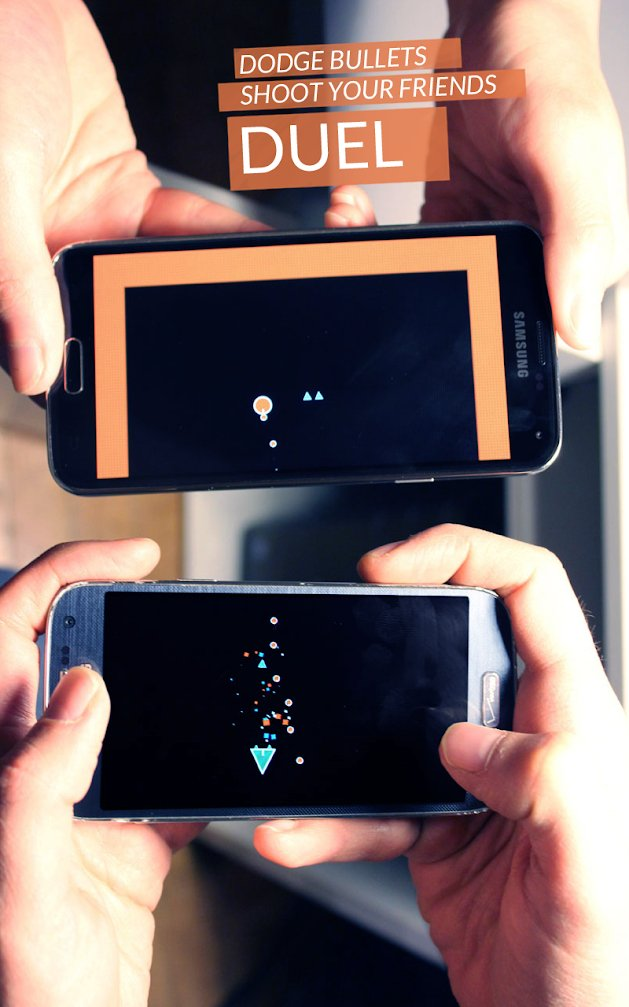
\includegraphics[width=0.5\linewidth]{assets/competitive-apps/dual.jpg}
    \caption{Screenshot hry DUAL!~\cite{seabaa_dual}}
    \label{fig:dual}
\end{figure}

První vybranou hrou je \emph{DUAL!}.
Tato hra využívá zejména prvky kooperace a rychlosti reakcí
a je velmi akčně laděná.
Jak říká první věta stránky hry v obchodě Google Play:
\todo{\emph{\uv{Between people, across screens.}}}~\cite{seabaa_dual}

Hra má několik módů.
Jedním z módů je mód \emph{DUEL}, ve kterém dva hráči
--- každý na svém zařízení ---
bojují proti sobě.
Hra obsahuje další 2 módy, které však nejsou přístupné zdarma,
proto zde nebudou zohledněny a popsány.

Herní plocha je rozdělena do dvou 2D částí.
Každý hráč se může pohybovat pouze ve své části, na svém zařízení.
Herní postava hráče se ovládá natáčením jeho displeje.
Postava má zásobník střel a po klepnutí na plochu postava vystřelí.
Při podržení se postupně ze zásobníku nabíjí střely
a vystřelí se větší, ale trochu pomalejší, střela.
Rychlým použitím gesta švihnutí se postava otočí.
Pokud hráč vystřelí na své ploše,
střela za chvíli doletí do protihráčovi části.
Střele protihráče se dá buď takticky vyhnout,
nebo zneškodnit vystřelením vlastní střely.

Cílem hry je několikrát zasáhnout protihráče, a tím ho zneškodnit.
Po ukončení hry je možné v dané relaci, s protihráčem, začít další kolo hry.

\subsection*{Klady}

\begin{itemize}
    \item UI je velmi jednoduché, avšak přívětivé svými barvami a srozumitelností.
    \item Hra je velmi krátká a dá se mnohokrát opakovat.
\end{itemize}

\subsection*{Zápory}

\begin{itemize}
    \item K dispozici zdarma je pouze jeden herní mód.
    \item Nejsou dostupné žádné speciální funkce, které by hru obohatily.
\end{itemize}
